\section{Accelerometer m�ling}\label{sec:bilag_acc}
Ved konstruering af et accelerometer er det vigtigt at montere den rette kondensator som afkobling. Ved de f�lgende fors�g er der monteret forskellige kondensator, og derefter er den data, microcontrolleren udsender, plottet som funktion af positionen. Banen, bilen k�rte p�, er vist p� Figur \ref{fig:bane}. Der er markeret ved tekstbokse fra A-D, som viser de forskellige sving. Disse kan derefter afl�ses p� de f�lgende grafer.

\begin{figure}[H]
	\begin{center}
	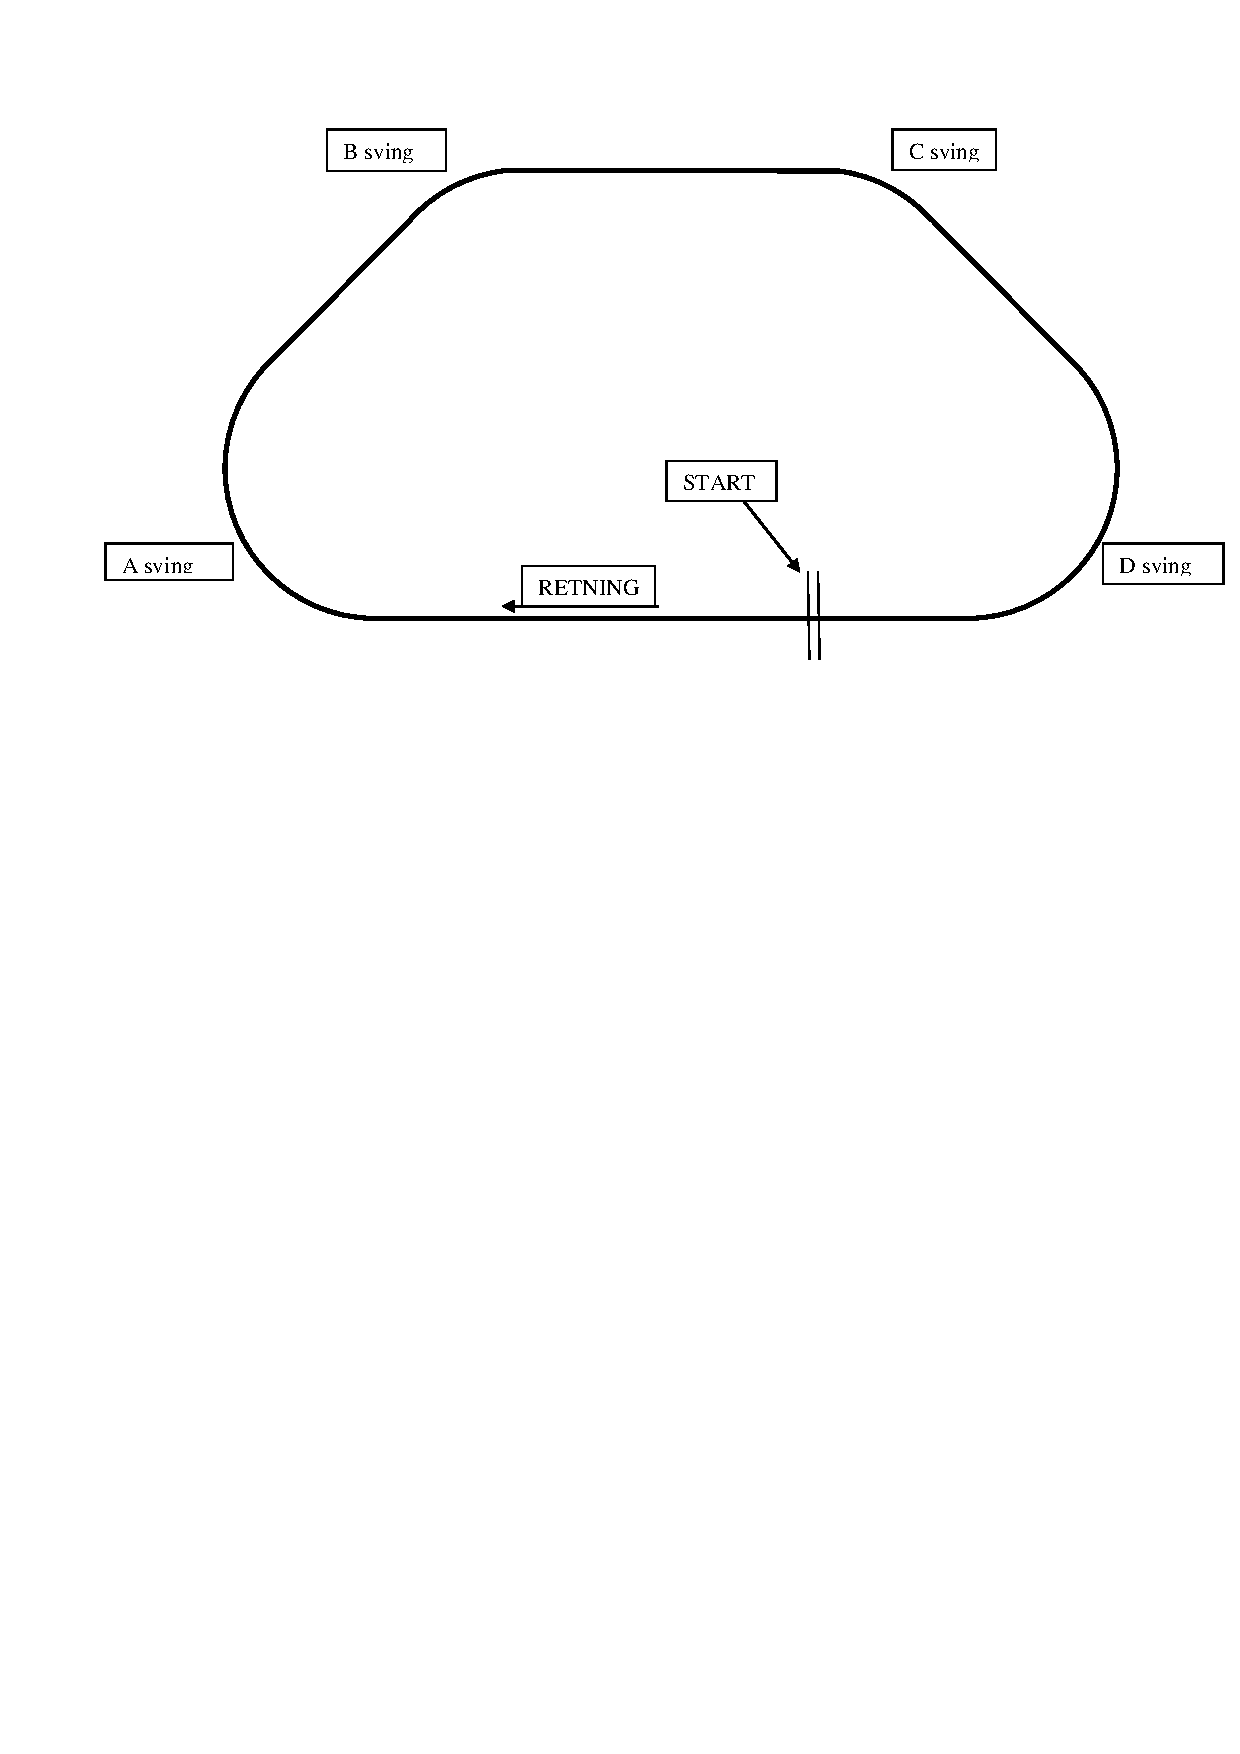
\includegraphics[scale=0.8,trim=40 520 0 50]{bane.pdf}%trim=l b r t
	\caption{Banen accelerometer-test blev udf�rt p�}
	\label{fig:bane}
	\end{center}
\end{figure}

Hvis ingen kondensator er monteret, er dataen accelerometeret sender ud, totalt ubrueligt. Derfor er der ikke tilf�jet A-D, da dataen er fuldst�ndig ubrugelig.  Det er vist p� Figur \ref{fig:acc0uftest0}, hvor bit-v�rdien er p� den lodrette akse og tiden er p� den vandrette akse.

\begin{figure}[H]
	\begin{center}
	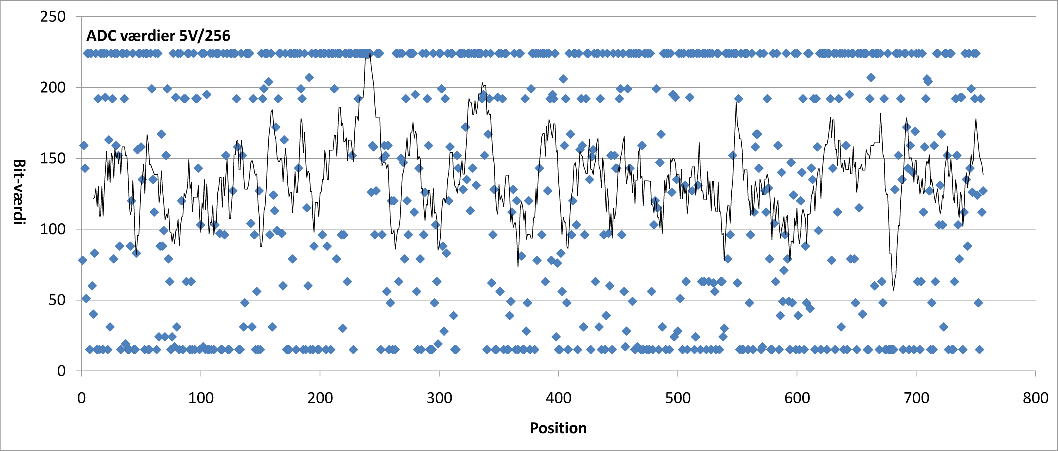
\includegraphics[scale=0.8]{acc_0uf_test0.pdf}%trim=l b r t
	\caption{Ingen kondensator monteret}
	\label{fig:acc0uftest0}
	\end{center}
\end{figure}

Der blev derefter monteret en 0,47$\mu$F kondensator og resultatet blev straks meget bedre - men stadig ikke tilfredsstillende. Man ser tydeligt, at den opfanger svingene, men stadig er mange v�rdier svingende. Dette ses p� Figur \ref{fig:acc_047uf_test2}

\begin{figure}[H]
	\begin{center}
	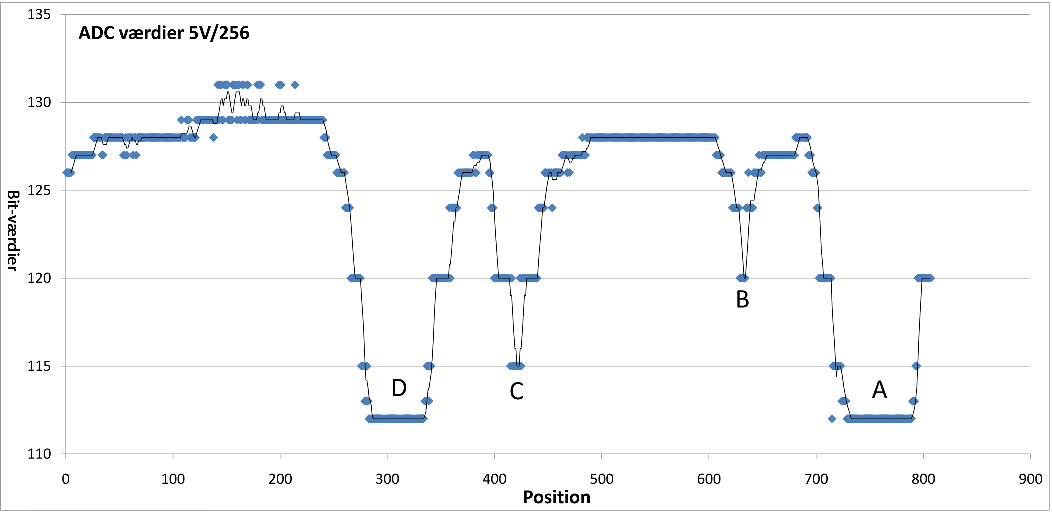
\includegraphics[scale=0.8]{acc_047uf_test2.pdf}%trim=l b r t
	\caption{0.47$\mu$F kondensator omvendt k�rsel}
	\label{fig:acc_047uf_test2}
	\end{center}
\end{figure}

For at kunne g�re m�lingerne mere pr�cise, m�tte en st�rre kondensator monteres som afkobling. Derfor blev en 1.0$\mu$F Kondensator monteret, og her blev resultatet rigtig godt. Som vist p� Figur \ref{fig:acc_1uf_test5}, ser man tydeligt, at alle sving bliver opfanget knivskarpt.

\begin{figure}[H]
	\begin{center}
	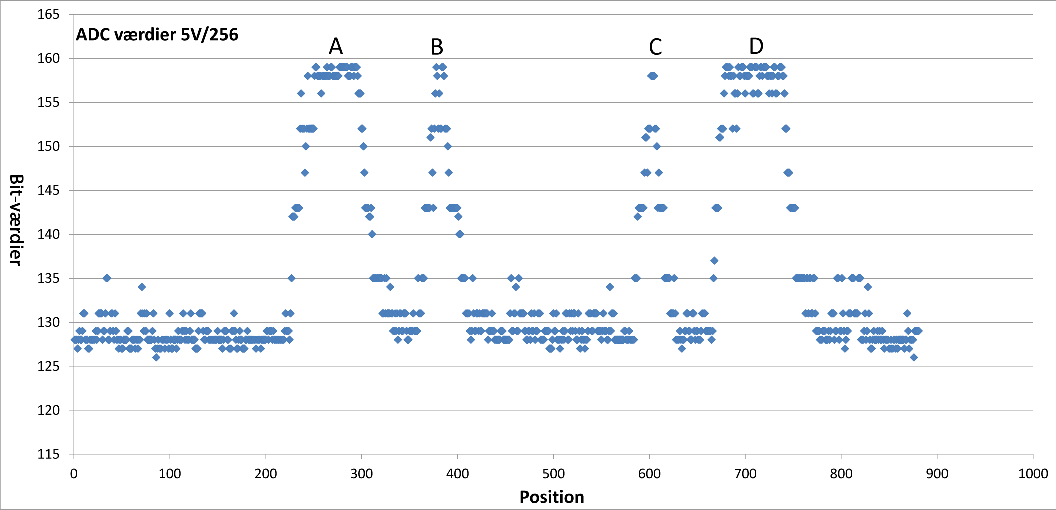
\includegraphics[scale=0.8]{acc_1uf_test5.pdf}%trim=l b r t
	\caption{1.0$\mu$F kondensator}
	\label{fig:acc_1uf_test5}
	\end{center}
\end{figure}

For at finde ud af om montering af en st�rre kondensator, ville give d�rligere eller bedre pr�cision, monteres der en 1.5$\mu$F kondensator. Som vist p� Figur \ref{fig:acc_1_5uf_test6} ses der, at resultaterne er rimelig pr�cise, men der bliver desv�rre sk�ret nogle af svingene af. Dette ses fx ved punkt C, der er sk�ret noget af acceleracionen af. Dette vil i sidste ende give store problemer. 

\begin{figure}[H]
	\begin{center}
	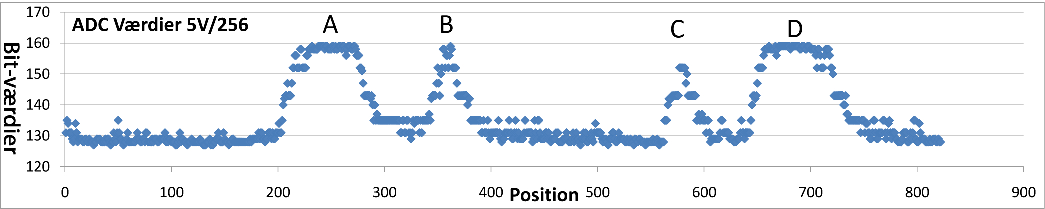
\includegraphics[scale=0.8]{acc_15uf_test6.pdf}%trim=l b r t
	\caption{1.5$\mu$F kondensator}
	\label{fig:acc_1_5uf_test6}
	\end{center}
\end{figure}

Som tidligere n�vnt blev 1.0$\mu$F den store vinder og derfor er denne monteret p� accelerometeret.